\subsection{\textit{Blockchain-Technologie}}

\subsubsection{Definition} \label{blockchain-definition}
Eine \textit{Blockchain} als Ganzes betrachtet, ist ein System zur Transaktionsabwicklung mit besonderen Eigenschaften. Als erstes beschrieben wurde die \textit{Blockchain} im Paper von \cite{Nakamoto2009} zur Realisierung der digitalen Währung \ac{btc}. Aus technischer Sicht gehört die \textit{Blockchain-Technologie} zum Bereich der verteilten Datenbanken. Ein \textit{Block} in einer \textit{Blockchain} repräsentiert eine Menge von Datensätzen die in der \textit{Blockchain} (Datenbank) vorgehalten werden. Jeder \textit{Block} (Datensatz) widerrum besitzt genau einen Vorgänger und einen Nachfolger. Allerdings werden diese Blöcke nicht wie in klassischen relationalen Datenbanksystemen in Tabellenstrukturen abgelegt und verwaltet. Durch die Vorgänger Information wird jeder neue Datensatz immer an den letzten Datensatz angehangen. Daraus bildet sich eine Kette von Blöcken - daher der Name \textit{Blockchain} (dt. Blockkette).

Ein \textit{Block} innerhalb der Kette kann definiert werden als verschlüsseltes Stück Information. Er beinhaltet neben den Transaktionen noch einen Zeitstempel und zwei kryptographische Hashwerte. Der erste Hashwert wird aus dem \textit{Block} selbst gebildet und der zweite Hashwert ist die Verknüpfung zum Vorgänger \citep{Tschorsch2016}. Wird nachträglich ein Wert einer Transaktion verändert oder ein ganzer \textit{Block} aus der Kette entfernt passt der jeweilige Hashwert des Vorgängers nicht mehr und durch den linearen Aufbau der \textit{Blockchain} würde diese Manipulation jederzeit unmittelbar bemerkt werden bei der Validierung von neuen Transaktionen. Die Daten in der \textit{Blockchain} sind somit vor unbefugter Veränderung geschützt. Als dezentrale Datenbank wird auf jedem Knoten des sich aufspannenden Netzwerks aus Teilnehmern der \textit{Blockchain} eine exakte Kopie\footnote{Es gibt Ausprägungen von \ac{dlt} Systemen bei denen sog. Light Nodes nur einen zeitlichen Abschnitt der Datensätze vorhalten, um neue Transaktionen validieren zu können. In der generellen Definition wird von sog. Full Nodes ausgegangen in denen stets alle Datensätze vorgehalten werden.} des Datenbestands vorgehalten. Diese dezentrale Struktur bedeutet, dass ein \textit{Blockchain} Netzwerk nicht unter der Kontrolle oder Regulierung einer einzelnen Entität steht. Jeder Teilnehmer kann eigenständig im Netzwerk agieren und es ist kein Zwischenhändler nötig \citep{Drescher2017, Meier2018}.

Wird von einem der Teilnehmer eine Transaktion ausgelöst, wird diese nicht durch einen Intermediär sondern durch das Netzwerk erfasst und verarbeitet (Abbildung \ref{fig:change-in-transaction-model-blockchain}). Ein neuer \textit{Block} wird erschaffen und validiert wie es durch das Konsensprotokoll festgelegt wird.

\begin{figure}[h!]
	\centering
	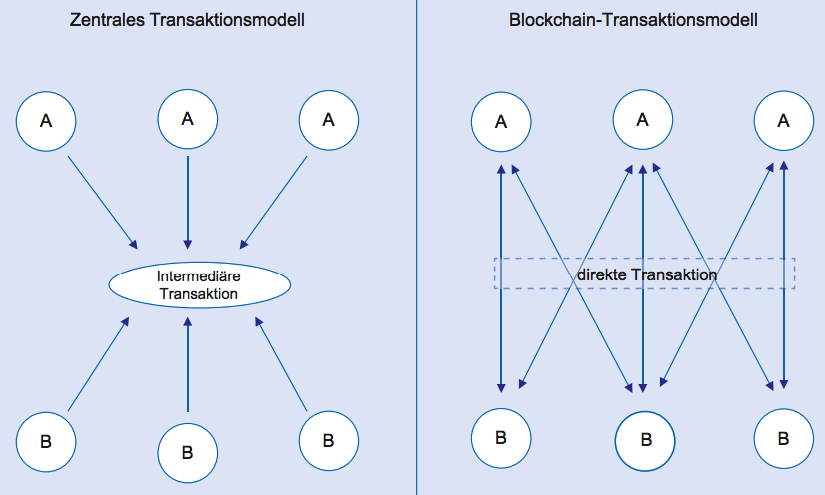
\includegraphics[width=1.0\linewidth]{pictures/change-in-transaction-model-blockchain}
	\caption[Transaktionsmodell Blockchain]{Transaktionsmodell Blockchain}
	\label{fig:change-in-transaction-model-blockchain}
\end{figure}

Dabei können solche \textit{Blockchain} Systeme ziemlich unterschiedlich ausgeprägt sein. Unterscheiden lassen sich diese Systeme zb. an der Art des Zugriffs, also wer darf Transaktionen lesen, wer darf sie schreiben. Außerdem kann der Mechanismus zur Konsensfindung je System anders sein.

% \citep{Abeyratne2016}
% \citep{Casino2019}

% \citep{Platzer2014}
% \citep{Narayanan2016}
% \citep{Burgwinkel2016}

% \citep{Gayvoronskaya2017}
% \citep{Vigna2017}
% \citep{JPMorgan2018}
% \citep{Buhl2017}
% \citep{Maull2017}
% \citep{Technik2018}
% \citep{Mitschele2018}
% \citep{Neugebauer2018}
% \citep{Min2018}


\subsubsection{Begriffliche Abgrenzung}

Die am häufigsten verwendeten Begriffe werden im Folgenden anhand eines Schichtenmodells (Abbildung \ref{fig:layer-model-blockchain}) erklärt und voneinander abgegrenzt.

\begin{figure}[h!]
	\centering
	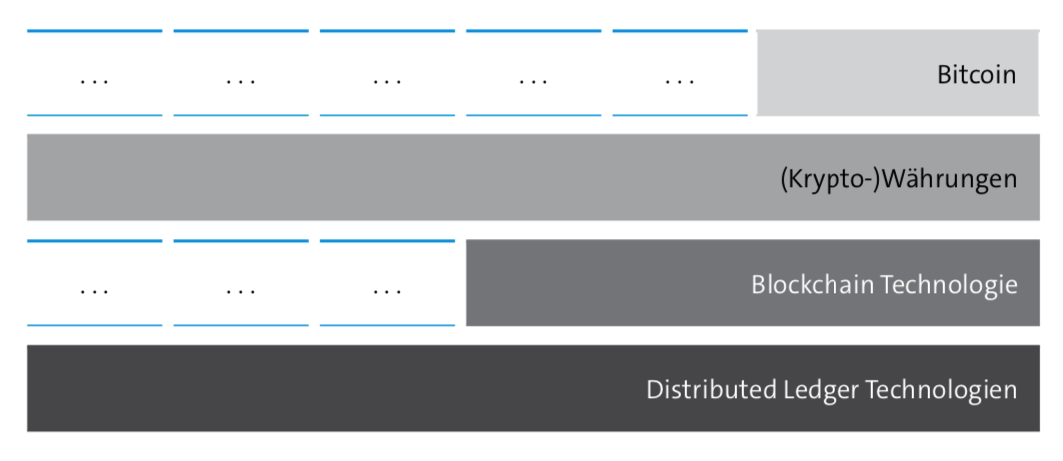
\includegraphics[width=1.0\linewidth]{pictures/layer-model-blockchain}
	\caption[Schichtenmodell \textit{Blockchain} Begriffe]{Schichtenmodell \textit{Blockchain} Begriffe QUELLE}
	\label{fig:layer-model-blockchain}
\end{figure}

\paragraph{Distributed Ledger}$~~$\\
Der \textit{Distributed Ledger} bildet die Basis des Schichtenmodells. Er ist im Grunde genommen ein klassisches Betandsbuch, das über einen Mechanismus verfügt, es auf alle teilnehmenden Parteien zu verteilen. \textit{Distributed Ledger} existieren bereits seit längerer Zeit und sind meist auf der technischen Basis einer verteilten Datenbank mit einer Logik auf Programm- oder Datenbankseite versehen, die aus der reinen Datenbank ein Bestandsbuch macht.

Distributed Ledger Technologie wird zunehmend synonym zum bisherigen Gebrauch von \textit{Blockchain} genutzt, um die Entwicklungen nach dem Bitcoin und den Kryptowährungen von eben diesen begrifflich abzugrenzen.

\paragraph{Blockchain-Technologie}$~~$\\
Die \textit{Blockchain} ist eine Form, einen \textit{Distributed Ledger} zu organisieren und zu implementieren. Auf die technische Implementierung der \textit{Blockchain} wird in den folgenden Kapiteln näher eingegangen; zur Begriffsbestimmung seien hier die grundlegenden Eigenschaften aufgezählt, die der \textit{Blockchain} in den letzten Jahren die steigende Aufmerksamkeit ermöglich haben:

\begin{itemize}
  \item Dezentralisiert
  \item Peer-to-Peer
  \item Transparenz und Anonymität
  \item Vertrauen
\end{itemize}

Blockchain gehört zu den bekanntesten Distributed-Ledger-Technologien. Aus diesem Grund wird die Bezeichnung Blockchain-Technologie in dieser Arbeit synonym für Distributed-Ledger-Technologien benutzt. Auf die technischen Eigenschaften von weiteren Ausprägungen der Distributed-Ledger-Technologien wird in dieser Arbeit daher nicht eingegangen.

\paragraph{Kryptowährungen}$~~$\\
Mit der \textit{Blockchain} als Basistechnologie lassen sich darauf aufbauende komplexe Systeme, wie z.B. Währungen abbilden. Wie in Kapitel \ref{blockchain-definition} erwähnt wurde die Blockchain-Technologie als erstes im Zusammenhang mit einer Kryptowährungen, dem Bitcoin, beschrieben. Die \textit{Blockchain} ist somit ein Nebenprodukt einer technischen Plattform, die eine kryptographische Währung erschuf und gleichzeitig ein System implementierte, um diese Währung zu nutzen und zu handeln.

Neben dem Bitcoin existiert eine Reihe weiterer Kryptowährungen, die sich zum Teil der dem Bitcoin zugrunde liegenden öffentlichen \textit{Blockchain} bedienen. Genannt seien hier z.B. Litecoin oder Dogecoin. Es existieren darüber hinaus Kryptowährungen, die eigene Blockchains zur Basis haben - zum Teil auf einer komplett eigenen technischen Implementierung. Vertreter hierfür sind z.B. Ethereum, Ripple oder Iota \citep[siehe auch][]{Buterin2014, carVertical, JPMorgan2018}.

\paragraph{Bitcoin}$~~$\\
Der Bitcoin ist die Kryptowährung, die auf der ursprünglichen \textit{Blockchain} gehandelt wird. Im Rahmen dieser Arbeit wird der Bitcoin und andere Kryptowährungen nicht weiter betrachtet.

\subsubsection{Arten von \textit{Blockchain}} \label{Arten-von-Blockchain}

Bei der Auswahl der Art einer \textit{Blockchain} trifft man auf zwei Widersprüche.

\begin{itemize}
  \item Transparenz vs. Vertraulichkeit
  \item Sicherheit vs. Geschwindigkeit
\end{itemize}

\paragraph{Transparenz vs. Vertraulichkeit}$~~$\\
Verwendet man eine \textit{Blockchain} werden Besitzverhältnisse durch die Transaktionshistorie ermittelt. Dabei lässt sie eine \textit{Blockchain} mit einem öffentlichen Register vergleichen. Im Sinne der Übertragung von Eigentum sind Offenheit und Transparenz zwei wesentliche Eigenschaften der Blockchain. Durch diese Offenheit ist jeder Teilnehmer in der Lage alle Transaktionen einzusehen und auf Manipulationen zu prüfen.

Dieses Vorgehen steht Gegensatz zur Vertraulichkeit die in bestimmten Bereichen unabdingbar ist. Durch Vertraulichkeit werden Informationen wie die Transaktionsdaten oder deren Details (beteiligte Konten oder transferierte Menge) vor unbefugter Einsicht geschützt. Hierdurch entsteht der Widerspruch zwischen Transparenz auf der einen Seite und Anforderungen an die Vertraulichkeit auf der anderen Seite \citep{Drescher2017}.

\paragraph{Sicherheit vs. Geschwindigkeit}$~~$\\
Die Datenstruktur einer \textit{Blockchain} sichert die Transaktionshistorie vor Manipulationen und Fälschungen. Jeder neue \textit{Block} der in der \textit{Blockchain} gespeichert werden soll muss vom Netzwerk durch das Lösen einer kryptographischen Aufgabe erzeugt und der Datenstruktur hinzugefügt werden. Dadurch ist es ziemlich aufwendig die Transaktionshistorie nachträglich zu manipulieren oder zu fälschen. Durch diesen Sicherheitsmechanismus sinkt die Geschwindigkeit mit der ein \textit{Blockchain} Netzwerk neue Transaktionen verarbeiten kann. Moderne Applikationen erfordern Geschwindigkeit und Skalierbarkeit was im direkten Kontrast zum erwähnten Sicherheitskonzept einer \textit{Blockchain} steht \citep{Drescher2017}.

\paragraph{Ursachen der Konflikte}$~~$\\
Zwei grundlegende Operationen eines \textit{Blockchain} Netzwerks sind Ursache für die beiden beschriebenen Widersprüche - Schreiben und Lesen von Transaktionsdaten. Der Konflikt zwischen Transparenz und Vertraulichkeit ist auf die Lese-Operationen einer \textit{Blockchain} zurückzuführen. Je offener die Leseberechtigungen einer \textit{Blockchain} sind, desto höher ist die Transparenz und desto niedriger ist die Vertraulichkeit der Transaktionsdaten. Die Schreib-Operationen sind für den Widerspruch zwischen Sicherheit und Geschwindigkeit verantwortlich. Je restriktiver die Berechtigungen zum Schreiben innerhalb des \textit{Blockchain} Netzwerks sind, desto höher ist die Geschwindigkeit mit der Transaktionen verarbeitet werden können. In Tabelle \ref{tab:technical-restricts-blockchain} werden die technischen Beschränkungen, der Widerspruch und die Operation innerhalb der \textit{Blockchain} zusammengefasst \citep{Drescher2017}.

\begin{table}[htb]\centering
  \begin{tabularx}{\textwidth}{XXX}
    \toprule
    \textbf{Beschränkung} &\textbf{Widerspruch} &\textbf{Blockchain Operation}\\ \midrule
    Keine Vertraulichkeit & Transparenz vs. Vertraulichkeit & Transaktionshistorie lesen\\ \addlinespace
    Skalierbarkeit & Sicherheit vs. Geschwindigkeit & Transaktionen schreiben\\
    \bottomrule
  \end{tabularx}
  \caption{Technische Beschränkungen der \textit{Blockchain} und ihre Ursachen}
  \label{tab:technical-restricts-blockchain}
\end{table}

\paragraph{Public vs. Private}$~~$\\
Betrachtet man die Berechtigungen zum Lesen innerhalb eines \textit{Blockchain} Netzwerks in der einfachsten Form muss das System zwischen Transparenz und Vertraulichkeit entscheiden. Entweder es werden allen Teilnehmern Leseberechtigungen zugeteilt oder nur einer ausgewählten Gruppe von Teilnehmern. Anhand des Kriterium, welcher Teilnehmer im Netzwerk neue Transaktionen erstellen und die Historie lesen kann, lässt sich eine \textit{Blockchain} als öffentliche oder private \textit{Blockchain} charakterisieren \citep{Drescher2017}.

\paragraph{Permissioned vs. Permissionless}$~~$\\
Die Schreibrechte bestimmen für ein \textit{Blockchain} Netzwerk den Grad der Skalierbarkeit. Werden Schreibrechte in ihrer einfachsten Form zugeteilt und alle Teilnehmer sind berechtigt Schreib-Operationen auszuführen, erhöht sich der Arbeitsaufwand je Teilnehmer der zur Berechnung nötigt wird. Dies ist für die Sicherheit des Netzwerk positiv, wirkt sich aber negativ auf die Geschwindigkeit aus. Durch die Geschwindigkeit wird das Netzwerk in der Skalierbarkeit beschränkt. Teilt man hingegen nur einer Gruppe von Teilnehmern Schreibrechte zu, ist der Arbeitsaufwand im Vergleich niedrig. Hierdurch kann das Netzwerk Transaktionen vergleichsweise schnell verarbeiten und ist dadurch selbst skalierbarer \citep{Drescher2017}.

\begin{figure}[h!]
	\centering
	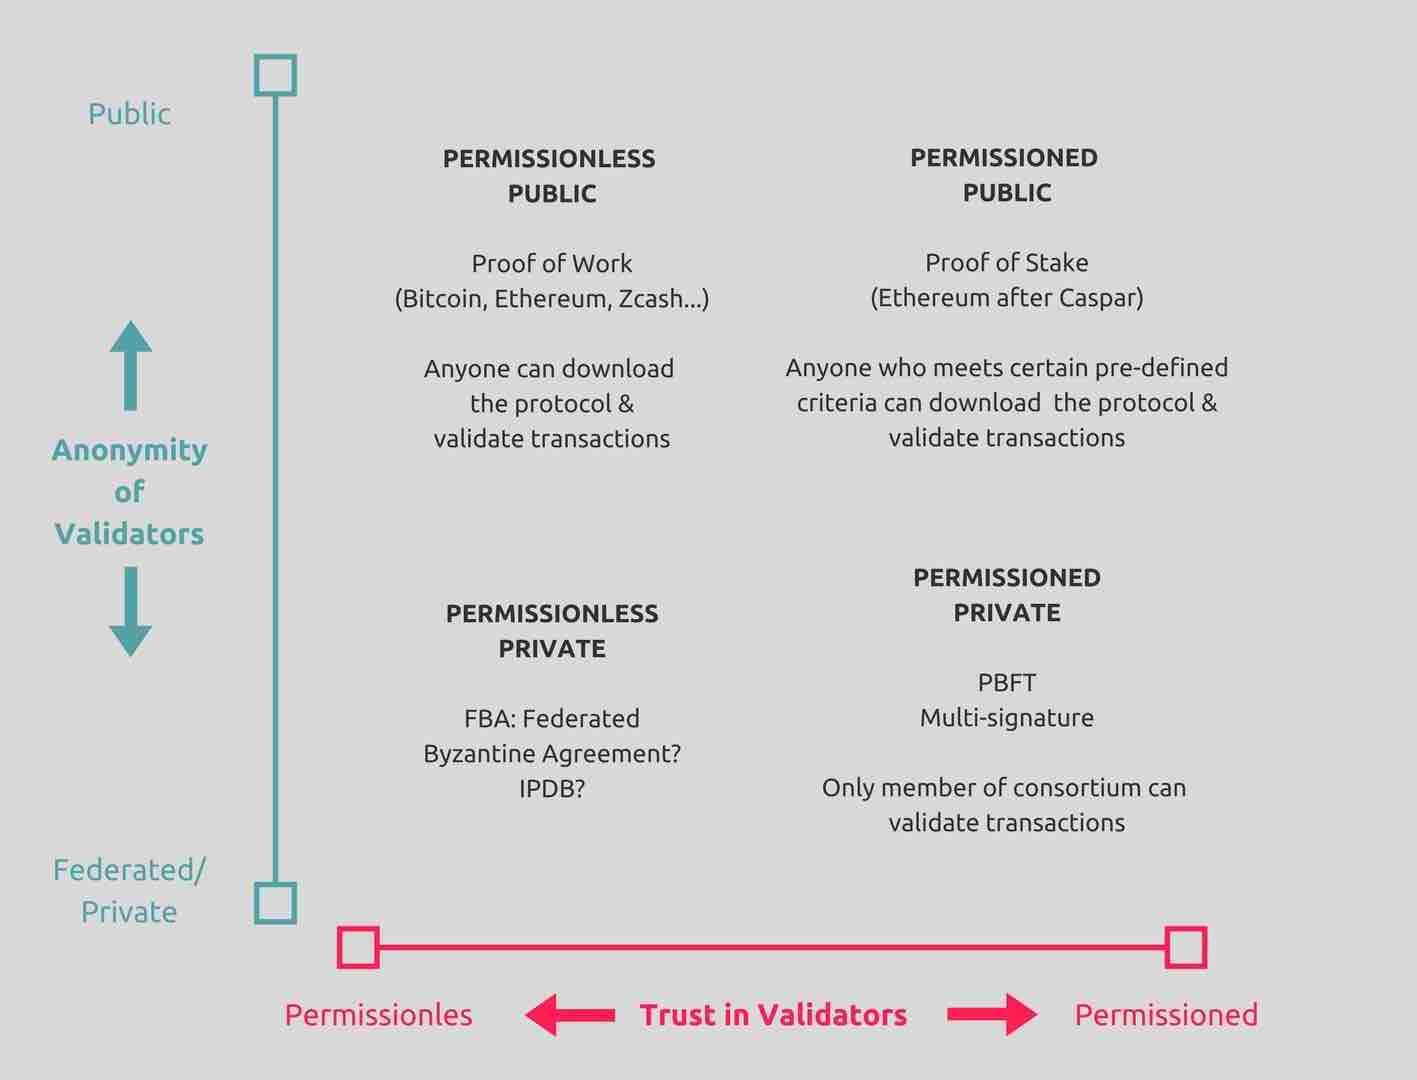
\includegraphics[width=1.0\linewidth]{pictures/dlt-type-matrix}
	\caption[Distributed Ledger Type Matrix]{Distributed Ledger Type Matrix ERSETZEN}
	\label{fig:dlt-type-matrix}
\end{figure}

\subsubsection{Technologischer Hintegrund}
Eine \textit{Blockchain} operiert auf einem \textit{Peer-to-Peer} Netzwerk in welchem jeder \textit{Knoten} eine exakte Kopie der Transaktionshistorie vorhält. Eine \textit{Blockchain} ist somit eine verteilte Datenbank, die eine kontinuierliche Liste von Transaktionen speichert und durch kryptographische Mechanismen vor Manipulation schützt. Transaktionen werden anhand eines Konsensusprotokolls validiert und zur Liste der Transaktionen hinzugefügt \citep{Nakamoto2009}.

\paragraph{Peer-to-Peer Netzwerke}$~~$\\
Ein \textit{Peer-to-Peer} Netzwerk ist der Gegensatz zum klassischen \textit{Client-Server-Modell}, bei dem ein \textit{Server} einen Dienst zur Verfügung stellt und ein oder mehrere \textit{Clients} diesen Dienst abrufen und nutzen. Bei einem \textit{Peer-to-Peer} Netz sind alle Teilnehmer, die sog. \textit{Peers}, gleichberechtigt und können Dienste anbieten und auch konsumieren. \textit{Peer-to-Peer} Netzwerke operieren als \textit{Overlay-Netze}\footnote{Ein \textit{Overlay-Netz} baut auf ein bestehendes Netz (\textit{Underlay Netz}) auf. Es kann mit eigenen Protokollen arbeiten und selbst als \textit{Underlay Netz} fungieren.\citep{Andersen2001}} auf dem Internet. Einige der häufigsten Eigenschaften von \textit{Peer-to-Peer} Netzwerken sind nach \citet{Steinmetz2005}:

\begin{itemize}
  \item Heterogenität zwischen den \textit{Peers} in Bezug auf Bandbreite, Rechenkraft und Speichergröße
  \item Qualität einzelner \textit{Peers} in Form von Verfügbarkeit und Verbindungsstärke lässt sich nicht voraussetzen
  \item Client-Server-Funktionalität wird für \textit{Peers} ermöglicht, um Dienste und Ressourcen anzubieten und zu konsumieren
  \item Austausch von Diensten und Ressourcen unter allen \textit{Peers} gewährleistet
  \item Bereitstellung von Such-Funktionen durch ein zusätzliches \textit{Overlay-Netz}
  \item Autonomie der \textit{Peers} in punkto Ressourcenbereitstellung
  \item Das \textit{Peer-to-Peer} Netzwerk organisiert sich selbst und nicht durch Dritte
\end{itemize}

\paragraph{Signierte Transaktionen durch Public-Key-Infrastruktur}$~~$\\
Wird eine Transaktion von einem Teilnehmer erstellt und soll durch das Netzwerk validiert werden kommen digitale Signaturen zum Einsatz. Digitale Signaturen gehören zur asymmetrischen Kryptographie und werden dazu verwendet die Urheberschaft und Integrität einer Nachricht oder im Falle der Blockchain einer Transaktion zu prüfen.

\citep{Beutelspacher2010}
\citep{Menezes1997}

// Schlüsselpaare (Unterschied Public- und Private-Key, öffentlich an privat/privat an öffentlich)\\
// Erstellen einer Signature\\
// Bild modellieren in anlehnung an Drescher2017\\
\begin{figure}[h!]
	\centering
	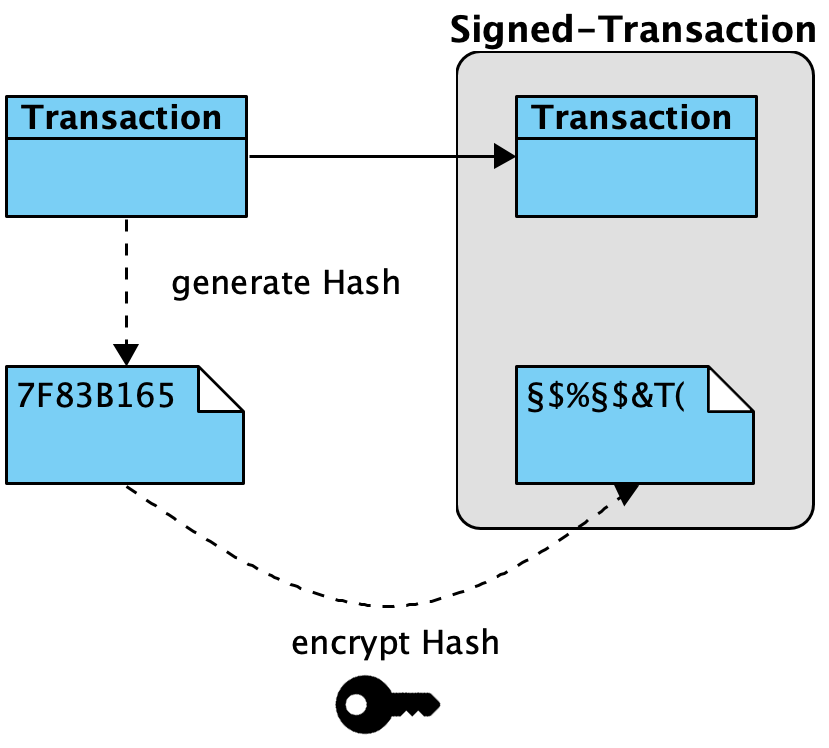
\includegraphics[width=0.5\linewidth]{pictures/digital-signatures-create}
	\caption[Erstellen einer digitalen Signatur]{Schematische Darstellung für das Erstellen einer digitalen Signatur}
	\label{fig:digital-signatures-create}
\end{figure}

// Prüfen einer Signatur\\
// Fall A Signatur ist korrekt -> Nachricht/Transaktion wurde nicht manipuliert UND Urheberschaft kann eindeutig zugeordnet werden
// Bild modellieren in anlehnung an Drescher2017\\
\begin{figure}[h!]
	\centering
	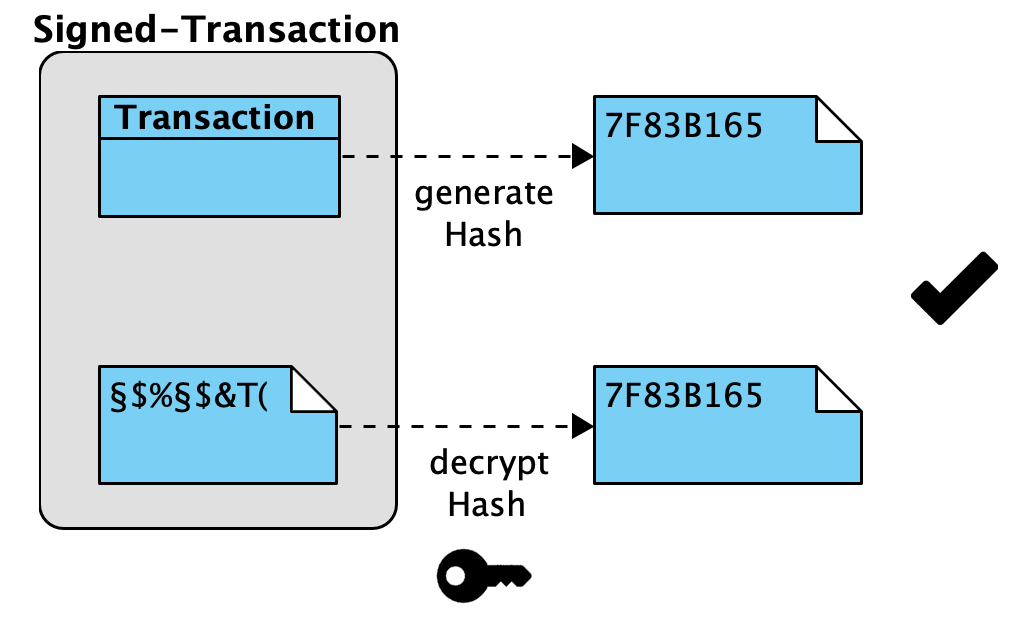
\includegraphics[width=0.5\linewidth]{pictures/digital-signatures-validate-positive}
	\caption[Prüfen einer digitalen Signatur]{Erfolgreiche Prüfung einer digitalen Signatur}
	\label{fig:digital-signatures-validate-positive}
\end{figure}

// Fall B Signatur ist nicht korrekt -> Nachricht/Transaktion wurde entweder manipuliert oder nicht vom angeblichen Urheber autorisiert
// Bild modellieren in anlehnung an Drescher2017\\
\begin{figure}[h!]
	\centering
	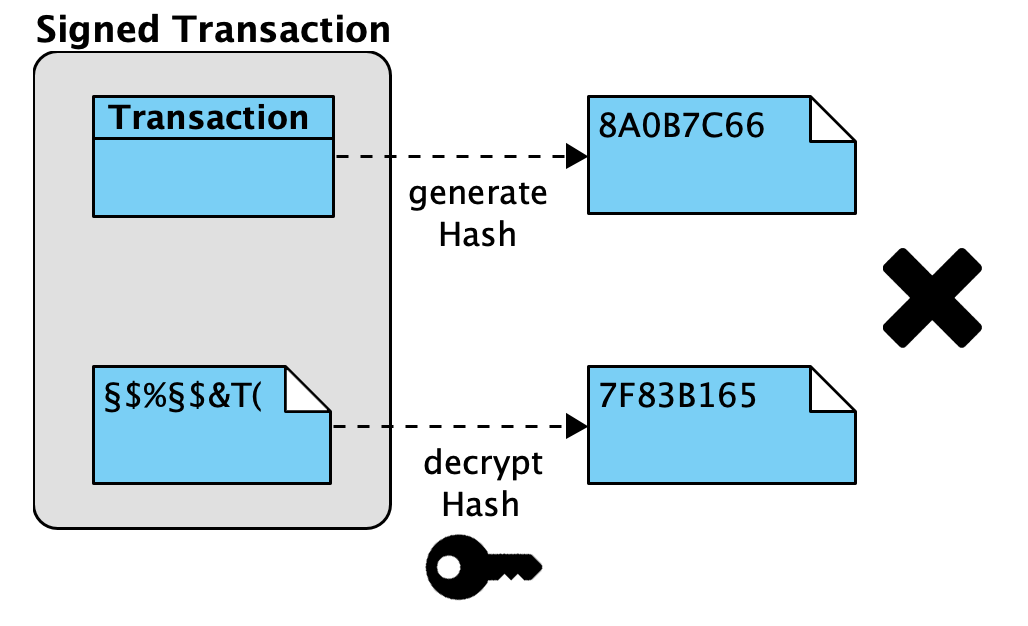
\includegraphics[width=0.5\linewidth]{pictures/digital-signatures-validate-negative}
	\caption[Manipulationerkennung durch digitale Signaturen]{Erkennung von Manipulation anhand der digitalen Signatur}
	\label{fig:digital-signatures-validate-negative}
\end{figure}

\paragraph{Kryptographisches Hashing}$~~$\\
Unterschied zwischen Hashing und krypt. Hashing aufzeigen. Matheformel :D
Evtl. die kleine Bilderreihe mit dem sich verändernden Hash Wert.
\citep{Menezes1997}
\citep{Diffie1976}

\paragraph{Konsensusprotokolle}$~~$\\
Byzantine Fault Tolerance erklären als Einstieg

Aufteilen nach Häufigkeit in der jeweiligen \textit{Blockchain} Art aus \ref{Arten-von-Blockchain}.
Ausschluss weiterer Betrachtung einiger Algorithmen für den weiteren Verlauf der Arbeit.


\subparagraph{Proof-of-X}$~~$\\
\begin{figure}[h!]
	\centering
	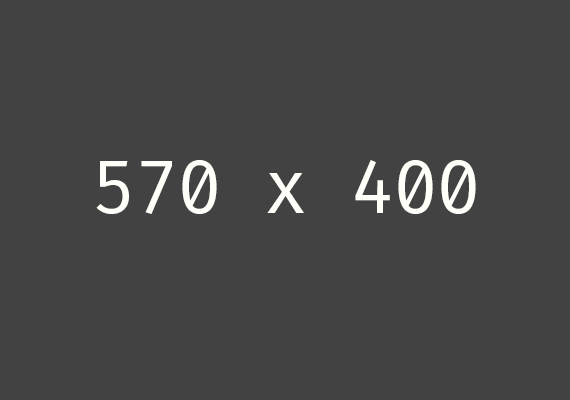
\includegraphics[width=1.0\linewidth]{pictures/placeholder_half_page}
	\caption[Placeholder Half Page]{Placeholder Half Page}
	\label{fig:placeholder_half_page}
\end{figure}

\subparagraph{Redundant Byzantine Fault Tolerance \& Plenum}$~~$\\
\begin{figure}[h!]
	\centering
	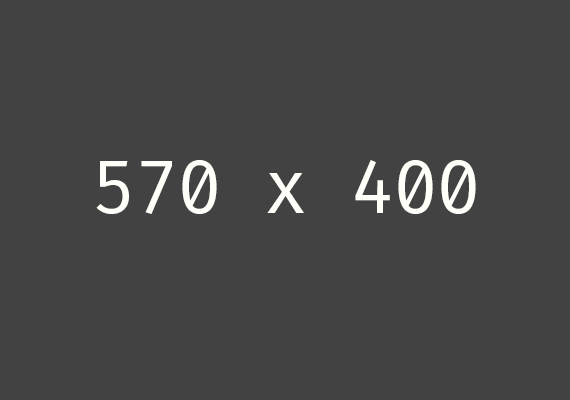
\includegraphics[width=1.0\linewidth]{pictures/placeholder_half_page}
	\caption[Placeholder Half Page]{Placeholder Half Page}
	\label{fig:placeholder_half_page}
\end{figure}
